
\chapter{Changes in 0.7.2}
\label{ch:072changes}
The 0.7.2 update release complements the releases of PharmML 0.7 \& 0.7.1,
in that it accounts for the missing description of design evaluation/optimisation tasks, see 
MCL specification \cite{Commets2015} and MCL examples \cite{CommetsExamples2015}.
These two tasks are now fully supported and described in some detail in section 
\ref{sec:newDesignTasks}.

At the same time a number of extensions has been made in ProbOnto knowledge 
base and ontology and more specifically we added new distributions/parameterisations 
and more then hundred properties and relationships between distributions. This is described 
in section \ref{sec:POextentions}. 

Few other changes are described in the last section. 


\section{New tasks -- design evaluation and optimization}
\label{sec:newDesignTasks}

The following listing exemplifies the available options in specifying an optimal 
design task additionally to those already available, see Figure \ref{fig:Flowchart_taskPart}. 
Covered are both sub-types: design evaluation and design optimisation tasks. 
The \xelem{OptimalDesignStep} element contains all relevant elements. 
The structure is therefore
\begin{itemize}
\item 
Simulation -- defined within \xelem{SimulationStep}
\item 
Estimation -- defined within \xelem{EstimationStep}
\item 
Optimal Design -- defined within \xelem{OptimalDesignStep}
\begin{enumerate}
\item 
Design Evaluation
\item
Design Optimisation
\end{enumerate}
\end{itemize}
Note, the that the information about the task's sub-type is stored within the 
\xelem{Operation} element. This allows to reuse existing structure and 
to remain consistent with previously supported \emph{Simulation} and 
\emph{Estimation} tasks. See section \ref{subsec:taskChoice} below is
explaining this in more details.
\begin{figure}[htb!]
\centering
 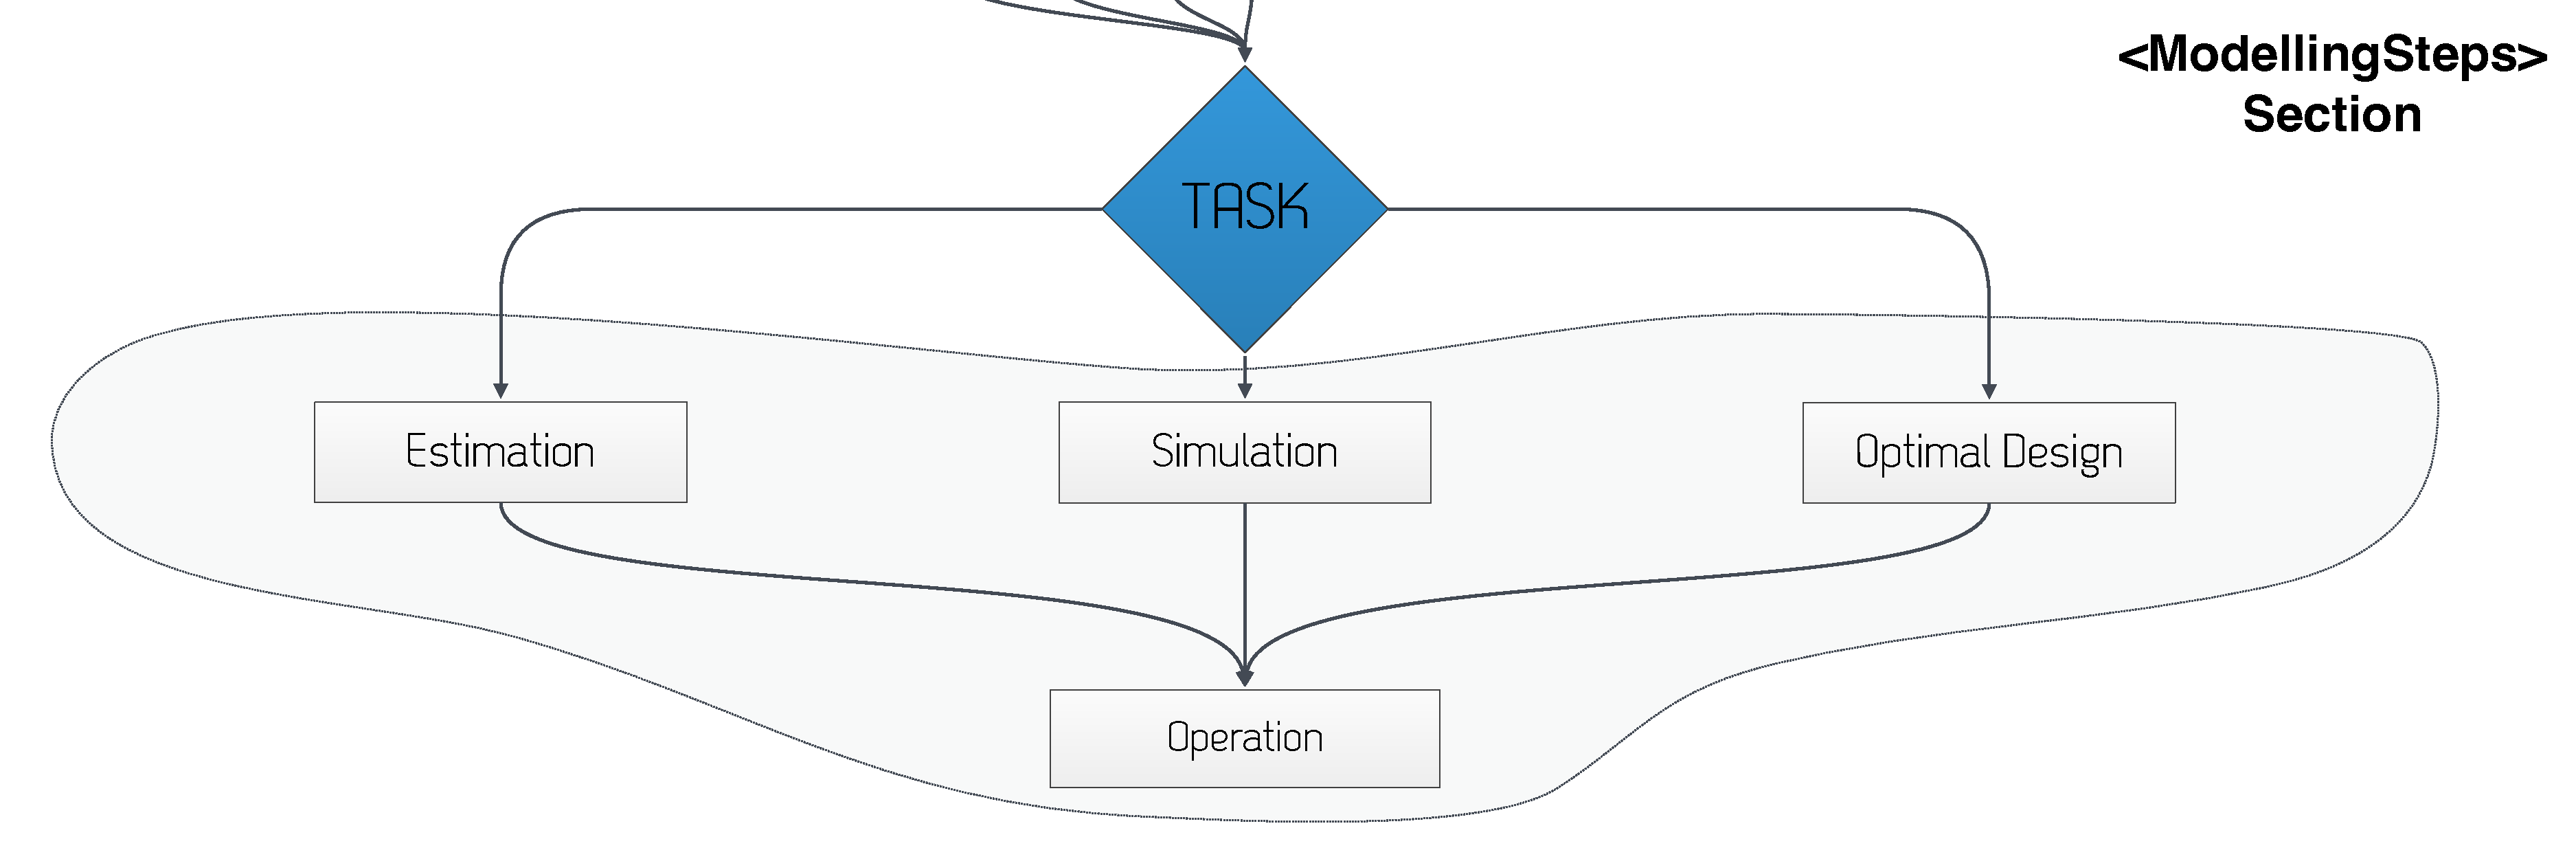
\includegraphics[width=140mm]{pics/Flowchart_stepsPart.pdf}
\caption{Flowchart with focus on the modelling steps -- the support for design 
evaluation and optimisation tasks, as part of the optimal design, is new in 
this release.}
\label{fig:Flowchart_taskPart}
\end{figure}
\newline
This section of PharmML starts with the opening tag
\lstset{language=XML}
\begin{lstlisting}
    <ModellingSteps xmlns="http://www.pharmml.org/pharmml/0.7/ModellingSteps">
\end{lstlisting}
after which one has the option to specify a target tool. In this case we declare 
PFIM as the target.
\lstset{language=XML}
\begin{lstlisting}
        <TargetTool oid="tTool">
            <TargetToolName>PFIM</TargetToolName>
        </TargetTool
\end{lstlisting}

In the following we will list all the available elements. IN general, not every 
element is required of course for every task -- the user defines what is 
needed). Because we talk about the design related tasks, we open their 
description with \xelem{OptimalDesignStep} and define the target tool reference 
first.
%\begin{itemize}
%\item 
%Optimal Design step
%\begin{itemize}
%\item 
%Reference to the target tool 
%\end{itemize}
%\end{itemize}

\subsubsection{XML template}
\lstset{language=XML}
\begin{lstlisting}
        <OptimalDesignStep oid="evaTask1">
            
            <TargetToolReference>
                <ct:OidRef oidRef="tTool"/>
            </TargetToolReference>
\end{lstlisting}


%%%%%%%%%%%%%%%%%%%%%%%%%%%%%%%%%%%%%%%%%%
\subsection{Optimization settings}
Although the \xelem{OptimiseOn} element is required for the optimisation task only, 
it is listed in this order in the MCL specification. We therefore keep the sequence 
and follow the same pattern. As the list below shows one can specify here 
any design element which can be used to define the optimisation:
\begin{itemize}
%\item 
%OptimiseOn
%\begin{itemize}
\item 
size of the arm 
\item  
dose amount
\item 
dosing times
\item 
infusion duration
\item 
number of design arms
\item 
number of samples
\item 
number of observation times
\item 
observation times
\item 
any other design element which can be referred to by an identifier, such as covariate or design parameter
%\end{itemize}
\end{itemize}

\subsubsection{XML template}
\lstset{language=XML}
\begin{lstlisting}
            <OptimiseOn>
                <ArmSize/>
                <DoseAmount>
                    <ct:Assign>
                        <ct:Real>100</ct:Real>
                    </ct:Assign>
                </DoseAmount>
                <DosingTimes/>
                <Duration/>
                <NumberArms/>
                <NumberSamples>
                    <ct:Assign>
                        <ct:Real>20</ct:Real>
                    </ct:Assign>
                </NumberSamples>
                <NumberTimes/>
                <ObservationTimes/>
                <ct:SymbRef symbIdRef="tdoseB"/>
                <ct:SymbRef symbIdRef="SEX"/>
            </OptimiseOn>
\end{lstlisting}

As apparent from the template above the specification of items to 
be optimised on can be limited to a list or can, in addition, contain an
assignment if an element of the design should be fixed to a specific
value, see for example \emph{dose amount} or \emph{number of 
samples}.

Another option is symbol reference, \xelem{SymbRef}, to point to a design 
parameter or covariate of interest.
\newline

%%%%%%%%%%%%%%%%%%%%%%%%%%%%%%%%%%%%%%%%%%
\subsection{FIM settings}
The specficaiton of FIM using a separate element is different compared to the 
original MCL specification \cite{Commets2015, CommetsExamples2015}.
The advantage is that once specified with a symbol identifier, the FIM can be 
referred to from the any subsequent element of the design task. There are following 
two options:
\begin{itemize}
\item 
Matrix or
\item 
File reference
\end{itemize}
FIM is either stored explicitly within the model file using the \xelem{Matrix} structure 
or in an external dataset as the following code snippet demonstrates.
\subsubsection{XML template}
\lstset{language=XML}
\begin{lstlisting}
            <FIM symbId="FIM1">
                <ct:Matrix matrixType="Any">
                    <ct:MatrixRow>
                        <ct:Real>1.1</ct:Real>
                        <!-- omitted elements -->
                        <ct:Real>1.6</ct:Real>
                    </ct:MatrixRow>
                        <!-- omitted rows -->
                    <ct:MatrixRow>
                        <ct:Real>10.1</ct:Real>
                        <!--omitted elements-->
                        <ct:Real>10.6</ct:Real>
                    </ct:MatrixRow>
                </ct:Matrix>
                <!-- ALTERNATIVE: FIM stored in an external file -->
                <!-- <File oid="FIMfile">
                    <ds:path>myFIM.csv</ds:path>
                </File>-->
            </FIM>
\end{lstlisting}


%%%%%%%%%%%%%%%%%%%%%%%%%%%%%%%%%%%%%%%%%%
\subsection{Method settings}
Once the FIM has been specified, the statistical criterion can be defined, which 
operates on that FIM. It can be either one of the common criterion, e.g. D, A, ...,
or an algebraic expression. For the latter there are again two options. Few 
frequently used build-in types can be selected, such as
\begin{itemize}
\item 
\xatt{det} which is equivalent to $det(FIM1)$
\item 
\xatt{logDet} which is equivalent to $log(det(FIM1))$
\item 
\xatt{trInv} which is equivalent to $tr(Inv(FIM1))$
\end{itemize}
with $FIM1$ defined above as the argument. Alternatively, any expression
can be provided. The following list shows these and other available options:
\begin{itemize}
\item 
Criterion: D, ED, ..., A
\item 
FIMfunction
\begin{itemize}
\item 
build-in types: det, logDet, trInv.
\item 
arbitrary expression
\end{itemize}
\item 
    ComputeFIM: FO. FOCE, ..., MCMC
\item 
    ApproximateFIM: full, ..., reducedParameterised
%            <xs:restriction base="xs:NCName">
%            <xs:enumeration value="full"/>
%            <xs:enumeration value="fullParamaterised"/>
%            <xs:enumeration value="block"/>
%            <xs:enumeration value="reduced"/>
%            <xs:enumeration value="reducedWithDerivative"/>
%            <xs:enumeration value="reducedParamaterised"/>
%            <xs:enumeration value="locModels"/>
%            <xs:enumeration value="switchModels"/>
%            <xs:enumeration value="weightedModel"/>
%            <xs:enumeration value="MCMC"/>
%        </xs:restriction>
\item 
    TypeFIM: individual, population, Bayesian 
\item 
    DesignType: exact, statistical
\item 
    Optimization Algorithm: simplex, fw
\end{itemize}
See the MCL specification,  \cite{Commets2015, CommetsExamples2015}, for 
the details.

\subsubsection{XML template}
\lstset{language=XML}
\begin{lstlisting}
            <Method>
                <Criterion type="A"/>
                <FIMfunction type="trInv">
                    <ct:Assign>
                        <math:MatrixUniop op="trace">
                            <math:MatrixUniop op="inverse">
                                <ct:SymbRef symbIdRef="FIM1"/>
                            </math:MatrixUniop>
                        </math:MatrixUniop>
                    </ct:Assign>
                </FIMfunction>
                <!--ALTERNATIVE for FIMfunction: 
                    using build-in operator types, here 'trInv' 
                    which is identical to the explicit expression 
                    above-->
                <!-- <FIMfunction type="trInv">     
                    <ct:Assign>
                        <ct:SymbRef symbIdRef="FIM1"/>
                    </ct:Assign>
                </FIMfunction>-->
                <ComputeFIM type="FO"/>
                <ApproximateFIM type="full"/>
                <TypeFIM type="population"/>
                <DesignType type="exact"/>
                <OptimizationAlgorithm type="FedorovWynn"/>
            </Method>
\end{lstlisting}


%%%%%%%%%%%%%%%%%%%%%%%%%%%%%%%%%%%%%%%%%%
\subsection{Cost settings}
The optimisation can be performed taking into account the design costs, expressed 
in various ways. Following options are available as: 
\begin{itemize}
\item 
TotalCost or
\item 
CostFunction
\begin{itemize}
\item 
build-in type: sample, individual
\item 
arbitrary expression
\end{itemize}
\end{itemize}

\subsubsection{XML template}
\lstset{language=XML}
\begin{lstlisting}
            <Cost>
                <TotalCost>
                    <ct:Assign>
                        <ct:Real>1.3</ct:Real>
                    </ct:Assign>
                </TotalCost>
                <CostFunction type="sample"/>
            </Cost>
\end{lstlisting}


%%%%%%%%%%%%%%%%%%%%%%%%%%%%%%%%%%%%%%%%%%
\subsection{Prior information settings}
Additionally to the criterion and method selections, one can specify any prior information
available, which can be provided as
\begin{itemize}
\item 
Matrix or
\item 
External File
\end{itemize}
and the following code snippet illustrates how this is implemented
\subsubsection{XML template}
\lstset{language=XML}
\begin{lstlisting}
            <PriorInformation>
                <ct:Matrix matrixType="Any">
                    <ct:MatrixRow>
                        <ct:Real>1.1</ct:Real><!--omitted_elements--><ct:Real>1.6</ct:Real>
                    </ct:MatrixRow>
                    <!-- omitted FIM rows -->
                    <ct:MatrixRow>
                        <ct:Real>10.1</ct:Real><!--omitted_elements--><ct:Real>10.6</ct:Real>
                    </ct:MatrixRow>
                </ct:Matrix>
                <!-- ALTERNATIVE to Matrix: prior information matrix stored 
                    in an external file -->
                <!-- <File oid="priorIMfile">
                    <ds:path>myPriorIM.csv</ds:path>
                </File>-->
            </PriorInformation>
\end{lstlisting}


%%%%%%%%%%%%%%%%%%%%%%%%%%%%%%%%%%%%%%%%%%
\subsection{Compute settings}
This section specifies which type of computations should be performed with their 
associated settings. For the majority of items a boolean value is sufficient, for others
an assignment of an interval or numerical values is required. 
\begin{itemize}
\item 
GraphOnly
\item 
PowerComparison
\item 
NSubjectComparison
\item 
PowerEquivalence
\item 
NSubjectEquivalence
\item 
EquivalenceRange
\item 
TypeIError
\item 
TypeIIError
\end{itemize}

\subsubsection{XML template}
\lstset{language=XML}
\begin{lstlisting}
            <Compute>
                <GraphOnly>
                    <ct:Assign>
                        <ct:False/>
                    </ct:Assign>
                </GraphOnly>
                <PowerComparison>
                    <ct:Assign>
                        <ct:True/>
                    </ct:Assign>
                </PowerComparison>
                <NSubjectComparison>
                    <ct:Assign>
                        <ct:True/>
                    </ct:Assign>
                </NSubjectComparison>
                <PowerEquivalence>
                    <ct:Assign>
                        <ct:Real>0.8</ct:Real>
                    </ct:Assign>
                </PowerEquivalence>
                <NSubjectEquivalence>
                    <ct:Assign>
                        <ct:True/>
                    </ct:Assign>
                </NSubjectEquivalence>
                <EquivalenceRange>
                    <ct:Assign>
                        <ct:Interval>
                            <ct:LeftEndpoint>
                                <ct:Assign>
                                    <math:Uniop op="log">
                                        <ct:Real>0.8</ct:Real>
                                    </math:Uniop>
                                </ct:Assign>
                            </ct:LeftEndpoint>
                            <ct:RightEndpoint>
                                <ct:Assign>
                                    <math:Uniop op="log">
                                        <ct:Real>1.2</ct:Real>
                                    </math:Uniop>
                                </ct:Assign>
                            </ct:RightEndpoint>
                        </ct:Interval>
                    </ct:Assign>
                </EquivalenceRange>
                <TypeIError>
                    <ct:Assign>
                        <ct:Real>0.05</ct:Real>
                    </ct:Assign>
                </TypeIError>
                <TypeIIError>
                    <ct:Assign>
                        <ct:Real>0.9</ct:Real>
                    </ct:Assign>
                </TypeIIError>
            </Compute>
\end{lstlisting}
Note that the \xelem{Interval} element has been introduced in PharmML 0.7
release, see section \ref{subsec:interval}.
\newline

%%%%%%%%%%%%%%%%%%%%%%%%%%%%%%%%%%%%%%%%%%
\subsection{Software settings}
\label{subsec:softSettings}
Target-specific tool settings can be stored in an external file -- 
this option is meant for settings which rarely change, compare next section 
\ref{subsec:taskChoice}.

\subsubsection{XML template}
\lstset{language=XML}
\begin{lstlisting}
            <SoftwareSettings>
                <File oid="softSettingsOID">
                    <ds:path>mySettings.xml</ds:path>
                </File>
            </SoftwareSettings>
\end{lstlisting}


%%%%%%%%%%%%%%%%%%%%%%%%%%%%%%%%%%%%%%%%%%
\subsection{Operation and choosing the task}
\label{subsec:taskChoice}

The last element of the design task description is complementary to the 
previously described software settings, section \ref{subsec:softSettings}.
The intension is to provide flexible storage place, using generic PharmML
elements available since version 0.2.1, allowing capturing of tool specific 
information. This can be altered directly in the model file without the necessity
to edit the settings stored in the external file.
The list shows some PFIM typical settings

\begin{itemize}
\item 
Operation
\begin{itemize}
\item
evaluation OR optimisation
\item 
Property, e.g. RtolEq, AtolEq, graph.logical, log.logical, graph.only, y.range
\end{itemize}
\end{itemize}

\subsubsection{XML template}
\lstset{language=XML}
\begin{lstlisting}
            <Operation opType="evaluation" order="1">
                <Property name="RtolEq">
                    <ct:Assign>
                        <ct:Real>1E-06</ct:Real>
                    </ct:Assign>
                </Property>
                <Property name="AtolEq">
                    <ct:Assign>
                        <ct:Real>1E-06</ct:Real>
                    </ct:Assign>
                </Property>
                <Property name="graph.logical">
                    <ct:Assign>
                        <ct:True/>
                    </ct:Assign>
                </Property>
                <Property name="log.logical">
                    <ct:Assign>
                        <ct:String>'y'</ct:String>
                    </ct:Assign>
                </Property>
                <Property name="graph.onf">
                    <ct:Assign>
                        <ct:Real>0</ct:Real>
                    </ct:Assign>
                </Property>
                <Property name="y.range">
                    <ct:Assign><ct:Interval>
                        <ct:LeftEndpoint>
                            <ct:Assign>
                                <ct:Real>0</ct:Real>
                            </ct:Assign>
                        </ct:LeftEndpoint>
                        <ct:RightEndpoint>
                            <ct:Assign>
                                <ct:Real>10</ct:Real>
                            </ct:Assign>
                        </ct:RightEndpoint>
                    </ct:Interval></ct:Assign>
                </Property>
            </Operation>
        </OptimalDesignStep>
\end{lstlisting}

%%%%%%%%%%%%%%%%%%%%%%%%%%%%%%%%%%%%%%%%%%%%%%%%%%%%%%
\subsection{Design example update}
All design examples, as described in 0.7 release, see section \ref{sec:designExamples},
have been updated will full task specification as formulated in the original MCL examples
document, \cite{CommetsExamples2015}.



%%%%%%%%%%%%%%%%%%%%%%%%%%%%%%%%%%%%%%%%%%%%%%%%%%%%%%
\section{Extensions/changes in ProbOnto}
\label{sec:POextentions}

The following list summarises the new development in ProbOnto
\begin{itemize}
\item 
New distributions have been added, see table \ref{figTable:univariates}, 
for example the Double Poiisson and additional parameterisations of 
generalised Poisson, negative binomial and log-normal distributions.
\item 
Negative Binomial -- changes in formulation for the NB1
have been made to account for the most common form used in the literature. 
See a detailed discussion in appendix \ref{app:sec:NB1discussion}.
\item 
More then 50 properties added, such as: linear combination, convolution, 
scaling, product, inverse, minimum, maximum, forgetfullness, residual, 
variate generation. See the excellent Leemis paper, \cite{Leemis:2008tg}, 
for definitions of these properties.
\item 
More then 30 relationships between various distributions, most of them as 
described in Leemis, \cite{Leemis:2008tg}, see also figure \ref{fig:POdiagram}.
\item 
About 40 re-parameterisations between the members of normal, log-normal, 
negative binomial and generalised Poisson distributions families. Also indicated
in the figure \ref{fig:POdiagram}.
\end{itemize}

\begin{figure}[htb!]
\centering
\begin{tabular}{cc}
 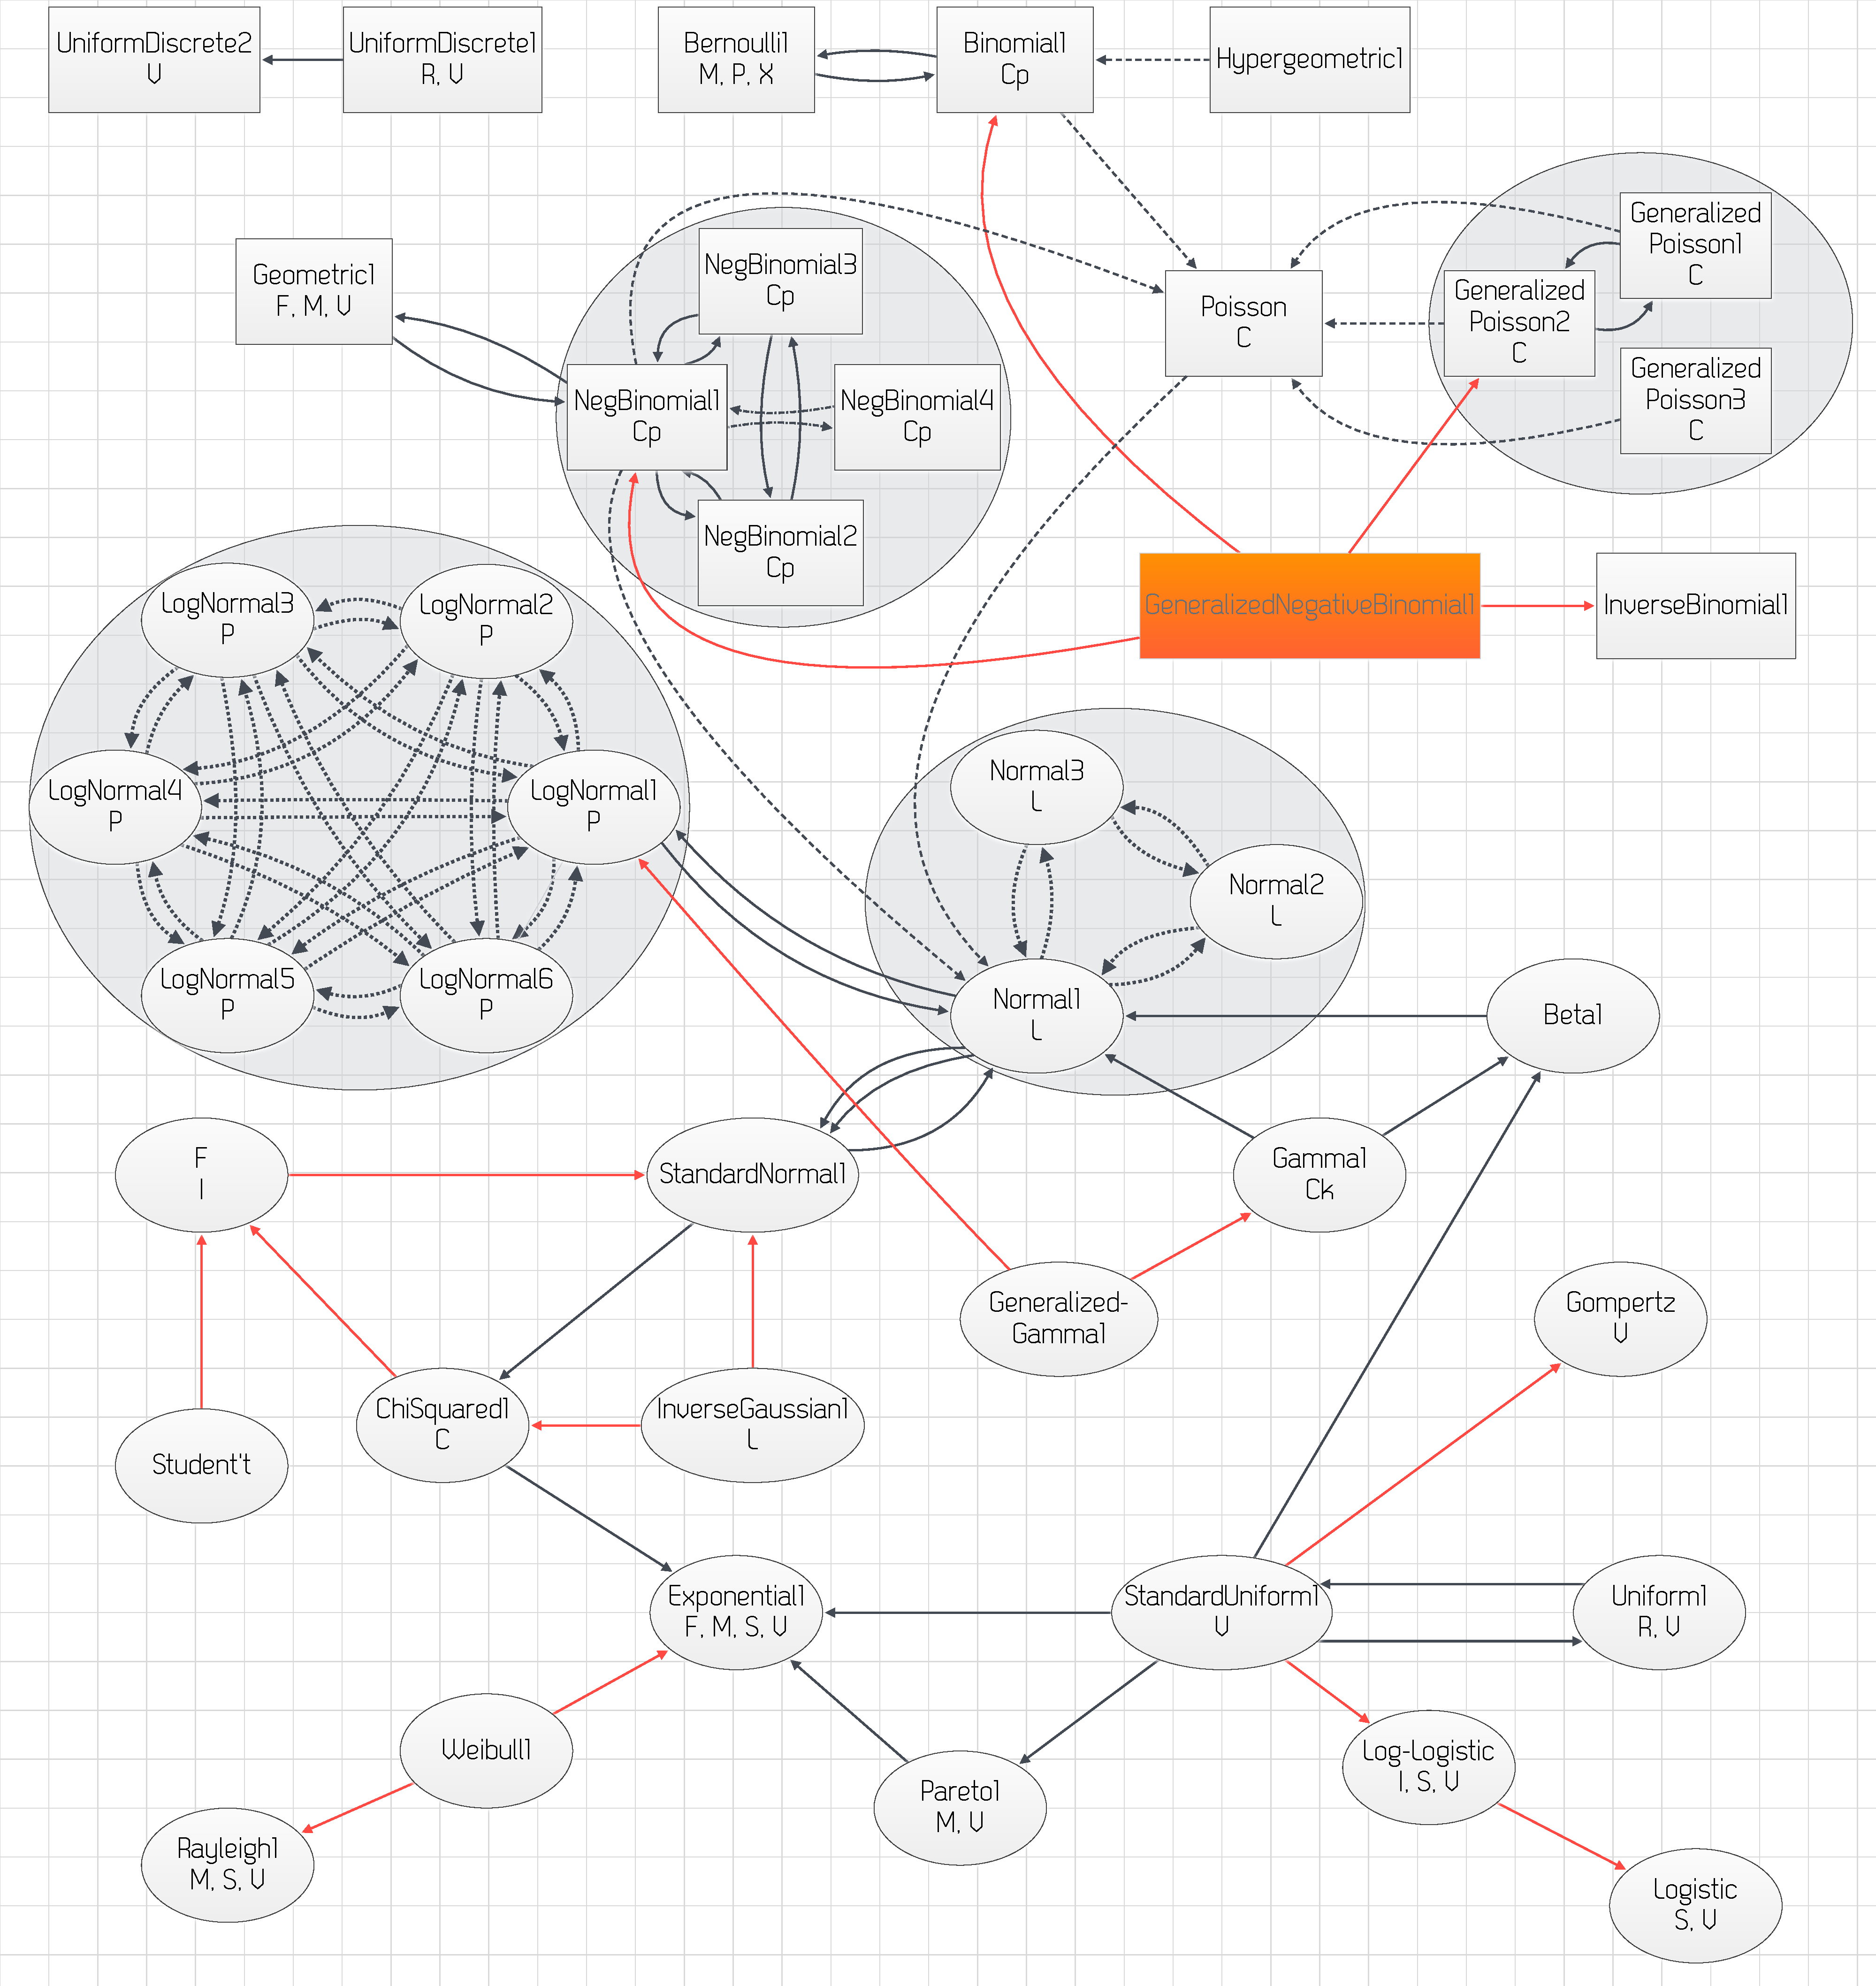
\includegraphics[width=160mm]{pics/POdiagram}
\end{tabular}
\caption{ProbOnto relationships diagram with selected distributions. 
Current ProbOnto version contains 70 relationships/re-parameterisations and 
more then 50 properties (indicated by the capitals in the according 
distribution box). Orange reletionship lines are under construction.}
\label{fig:POdiagram}
\end{figure}

\subsection{Count data models support}
\label{subsec:countModels}
Growing number of count data related distributions means better coverage 
of this important type of models, \cite{Paule:2012fk, Plan:2014kq}. 
The models supported so far include
\begin{itemize}
\item 
Double Poisson ($\mu, \phi$)
\item 
Generalized Poisson
\begin{itemize}
\item 
Generalized Poisson 1 ($\theta, \delta$)
\item 
Generalized Poisson 2 ($\mu, \delta$)
\item 
Generalized Poisson 3 ($\mu, \alpha$)
\end{itemize}
\item 
Inverse Binomial ($k, p$)
\item 
Negative Binomial 
\begin{itemize}
\item 
Negative Binomial 1(\emph{r, p})
\item 
Negative Binomial 2 ($\lambda, \tau$)
\item 
Negative Binomial 3 	($\mu, k$)
\item 
Negative Binomial 4 	($r,p$)
\end{itemize}
\item 
Poisson ($\lambda$)
\item 
Zero-Inflated Negative Binomial ($\lambda, \tau, p0$)
\item 
Zero-Inflated Poisson ($\lambda, \pi$)
\end{itemize}
As can be seen from the listing, two models come with multiple 
parameterisations. This aspect is described in detail in section 
\ref{sec:altParams}. 
In short,  their presence, with where available re-parameterisation formulas,
allows for accounting for and dealing with varying support in target tools.
The re-parameterisation formulas will be supported by the libPharmML
making model translation to the desired format an easy task. 

%See an analogous discussion on parameters differences between BUGS
%and R, \cite{lebauer2013translating}), which state that "[...] R and BUGS 
%languages use different representations of common probability density 
%functions, creating a potential for errors to occur in the implementation 
%or interpretation of analyses that use both languages".

\subsection{Bug fixes}
\begin{itemize}
\item 
Binomial distribution -- \xatt{numberOfTrials} instead of \xatt{numberOfFailures}
in table \ref{figTable:univariatesCodes}.
\end{itemize}

%
%\section{Time-to-Event modeling}
%
%Hazard/survival function added to mode common models
%\begin{itemize}
%\item 
%Weibull
%\item 
%Exponential
%\item 
%Rayleigh
%\item 
%Gompertz 
%\item 
%Lognormal
%\end{itemize}


%\section{Removing redundant elements}
%Removing parameter elements -- not used and not required
%IntensityParameter

        
\section{Other changes}
\label{sec:otherChanges072}
\begin{itemize}
\item 
A vector can be empty, i.e. when its elements are uniquely defend using the 
\xatt{default} and \xatt{length} attributes, similarly to what is possible when defining matrices. 
With this feature a \emph{null} vector, one whose all elements are zero,
can be simply specified.

One such use case can be found in the example \emph{orangeTrees\_MVN.xml} 
when defining the initial estimate of the mean vector $mean = c(0, 0, 0)$. 
Instead of listing all $0$'s explicitly, see following table (links), specifying vector's 
content and dimension with the according attributes provides the
complete information about it.

\begin{table}[ht!]
\setlength{\tabcolsep}{10pt}
\begin{center}
\begin{tabular}{cc}
  \hline
  \hline
\pml $\le$ 0.7.1  &  \pml 0.7.2 \\
  \hline
  \lstset{language=XML}
\begin{lstlisting}
<mstep:InitialEstimate>
    <ct:Vector>
        <ct:VectorElements>
            <ct:Real>0</ct:Real>
            <ct:Real>0</ct:Real>
            <ct:Real>0</ct:Real>
        </ct:VectorElements>
    </ct:Vector>
</mstep:InitialEstimate>
\end{lstlisting}
&
\lstset{language=XML}
\begin{lstlisting}
<mstep:InitialEstimate>
    <ct:Vector default="0" length="3"/>
</mstep:InitialEstimate>
\end{lstlisting}  \\
  \hline
  \end{tabular}
\vspace{-1.5em}
\label{tab:simplerVectors}
\end{center}
\end{table}

\item
\xatt{determinant} -- new matrix operator added which can be used e.g. 
to define the FIM function
\lstset{language=XML}
\begin{lstlisting}
               <FIMfunction>
                    <ct:Assign>
                        <math:MatrixUniop op="determinant">
                            <ct:SymbRef symbIdRef="FIM1"/>
                        </math:MatrixUniop>
                    </ct:Assign>
                </FIMfunction>
\end{lstlisting}
\item
Added several \xatt{columnType} attribute values to be used in SO for
the various scale of random effects, such as
\begin{itemize}
\item
\emph{randEffect\_stdev}, \emph{randEffect\_var}, \emph{randEffect\_cov}, 
\emph{randEffect\_corr} to account for various scales the random effects 
can be define on. 
\end{itemize}
\item
\xatt{inputTarget} attribute is now optional. This attribute functioned so far 
merely as an annotation in the dosing model and was not used by any target tool. 
It has been downgraded in that it's use can be decided by the user.
\item
Corrections in \emph{orangeTrees\_MVN.xml} model. If the type of a
matrix is specified as a diagonal one, i.e. \xatt{matrixType="Diagonal"} then the 
specification of the off-diagonal elements, e.g. \xatt{offDiagDefault="0.0E1"}
is redundant and has been removed from the example. 
In this particular case the implementation of the matrix, here in winBUGS language
\lstset{language=MLX}
\begin{lstlisting}
         prec = structure(.Data = c(1.0E-6, 0, 0,
                                       0, 1.0E-6, 0,
                                       0, 0, 1.0E-6), .Dim = c(3, 3)))
\end{lstlisting}
can be simplified further in that instead of 
\lstset{language=XML}
\begin{lstlisting}
<mstep:ParameterEstimation>
    <ct:SymbRef symbIdRef="prec"/>
    <mstep:InitialEstimate fixed="true">
        <ct:Matrix matrixType="Diagonal">
            <ct:MatrixRow><ct:Real>1.0E-6</ct:Real></ct:MatrixRow>
            <ct:MatrixRow><ct:Real>1.0E-6</ct:Real></ct:MatrixRow>
            <ct:MatrixRow><ct:Real>1.0E-6</ct:Real></ct:MatrixRow>
        </ct:Matrix>
    </mstep:InitialEstimate>
</mstep:ParameterEstimation>
\end{lstlisting}
we can simply define it as
\lstset{language=XML}
\begin{lstlisting}
<mstep:ParameterEstimation>
    <ct:SymbRef symbIdRef="prec"/>
        <ct:Matrix matrixType="Diagonal" numbCols="3" numbRows="3" diagDefault="1.0E-6"/> 
    </mstep:InitialEstimate>
</mstep:ParameterEstimation>
\end{lstlisting}
\end{itemize}
with attribute \xatt{numbCols} and \xatt{numbRows} specifying the matrix dimension.
While this is a low dimension matrix, this notation means a significant simplification
for higher dimensional cases.













